In \cite{Reid} and \cite[Appendix]{drazin-reid} the authors introduce generalized Airy functions $A_k, B_0, B_k$, $k=1,2,3$ as approximate solutions of the Orr--Sommerfield fluid equation. They are defined as contour integral \cite[Section 9.13(ii)]{dlmf}

\begin{align*}
\mathrm{A}_k(y,p)&=\frac{1}{2\pi i}\int_{\Gamma_k}e^{yt-\tfrac{t^3}{3}}\frac{dt}{t^p} \qquad k=1,2,3\,\, p\in\C \\
\mathrm{B}_0(y,p)&=\frac{1}{2\pi i}\int_{\Gamma_0}e^{yt-\tfrac{t^3}{3}}\frac{dt}{t^p} \qquad p\in\Z \\
\mathrm{B}_k(y,p)&=\int_{\gamma_k}e^{yt-\tfrac{t^3}{3}}\frac{dt}{t^p} \qquad k=1,2,3\,\, p\in\Z 
\end{align*}
where the contours $\Gamma_k, \Gamma_0, \gamma_k$ are represented in Figure \ref{fig:path-generalized-Airy}. 
\begin{figure}[ht]
\center
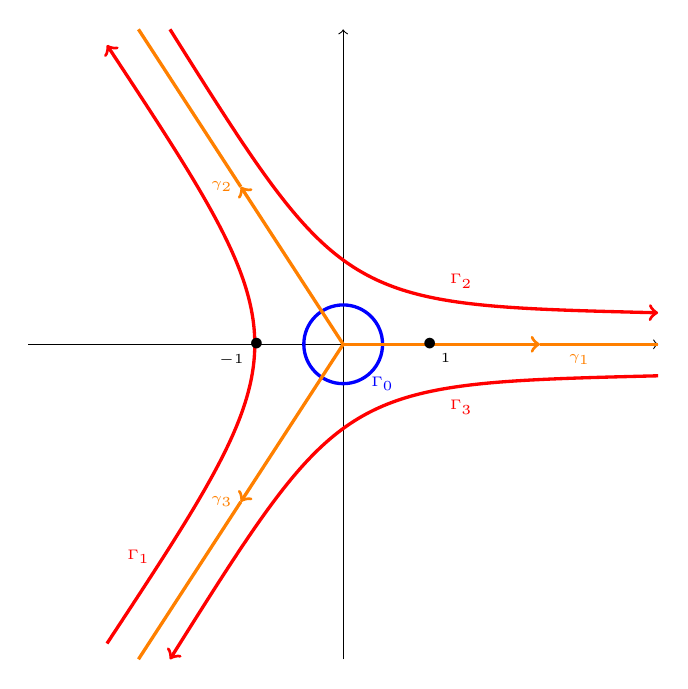
\begin{tikzpicture}
    \draw[->] (4,0)--(4,8);
    \draw[->] (0,4)--(8,4);
    \draw[blue,very thick] (4,4) circle (0.5) ;
    \node[blue,font=\tiny] at (4.5,3.5) {$\Gamma_0$};
    \node[red,font=\tiny] at (1.4,1.3) {$\Gamma_1$};
    \draw[red,very thick,->] (1,0.2) .. controls (3.5,4) .. (1,7.8);
    \node[red,font=\tiny] at (5.5,4.8) {$\Gamma_2$};
    \draw[red,very thick,->] (1.8,8) .. controls (4,4.5) ..(8,4.4) ;
     \node[red,font=\tiny] at (5.5,3.2) {$\Gamma_3$};
    \draw[red,very thick,->] (8,3.6) .. controls (4,3.5) ..(1.8,0) ;
    \draw[orange,very thick,->] (4,4)--(6.5,4);
    \draw[orange,very thick] (6.5,4)--(8,4);
    \node[orange,font=\tiny,below] at (7,4) {$\gamma_1$};
    \draw[orange,very thick,->] (4,4)--(2.7,6);
    \draw[orange,very thick] (2.7,6)--(1.4,8);
    \node[orange,font=\tiny,right] at (2.2,6) {$\gamma_2$};
    \draw[orange,very thick,->] (4,4)--(2.7,2);
    \draw[orange,very thick] (2.7,2)--(1.4,0);
    \node[orange,font=\tiny,right] at (2.2,2) {$\gamma_3$};
    \node at (5.1,4) {$\bullet$};
    \node at (2.9,4) {$\bullet$};
    \node[font=\tiny,below,right] at (2.3,3.8) {$-1$};
    \node[font=\tiny,below] at (5.3,4) {$1$};
    \end{tikzpicture}
    \caption{Representation of the path of integration for $\mathrm{A}_k,\mathrm{B}_0,\mathrm{B}_k$ respectively in red, blue and orange.}\label{fig:path-generalized-Airy}
\end{figure}

Each generalized Airy function is a solution of
\begin{equation}
\left[\partial_y^3-y\partial_y+(p-1)\right]f=0
\end{equation} 
and if $p=0$ they reduce to the classical Airy functions.

Following the treatment of the Airy--Lucas functions, we'll rewrite the generalized Airy function $\mathrm{A}_1(y,p)$ as thimble integrals with the function $f=4u^3-3u$. This follows from the change of coordinates $z=\tfrac{2}{3}y^{3/2}$, and gives $\mathrm{A}_1(y,p) = (12 z)^{\tfrac{1-p}{3}}\, I_+(z,p)$ with 
%
\[I_+(z,p):=\frac{1}{2\pi i}\int_{z^{-1/3}\Gamma_1} e^{-z(4u^3-3u)} \frac{du}{u^p}\]
%
\begin{verify}
  \begin{align*}
I_{+}(z,p)&=\frac{1}{2\pi i}\int_{\Lambda_{+}}e^{-z(4u^3-3u)}\, \frac{du}{u^p} &\\
&=\frac{1}{2\pi i}(12 z)^{(p-1)/3}\int_{z^{1/3}\Lambda_{+}}e^{-z(\tfrac{4}{12}\tfrac{t^3}{z}-3 (12 z)^{-1/3}t)}\frac{dt}{t^p} & u=(12 z)^{-\tfrac{1}{3}}t\\
&=\frac{1}{2\pi i}(12 z)^{(p-1)/3}\int_{z^{1/3}\Lambda_{+}}e^{-\left(\frac{t^3}{3}-(\tfrac{3}{2} z)^{2/3}t\right)}\frac{dt}{t^p} & \\
&=(12 z)^{(p-1)/3}\mathrm{A}_1((\tfrac{3}{2}z)^{2/3},p)
\end{align*}  
\end{verify}
%
Notice that, the critical points of $f$ are $\alpha_{\pm}=\pm\tfrac{1}{2}$, as in the Airy case. However, the volume form $\nu_p$ is meromorphic, hence $f$ should be regarded as a function from $\C^*$ to $\C$.     
%\begin{equation}
%I_\pm(z,p)\defeq\frac{1}{2\pi i}\int_{\Lambda_{\pm}}e^{-z(4t^3-3t)}\frac{dt}{t^p}
%\end{equation}
%where $\Lambda_{+}=z^{-1/3}\Gamma_1$ and $\Lambda_-=z^{-1/3}\Gamma_2$ are the paths through the points $\alpha_\pm$, starting and ending at infinity (as in Figure \ref{fig:path-generalized-Airy-Lambda+-}).
%\begin{figure}
%\center
%\begin{tikzpicture}
%    \draw[->] (4,0)--(4,8);
%    \draw[->] (0,4)--(8,4);
%    \node[red,font=\tiny] at (1.4,1.3) {$\Lambda_-$};
%    \draw[red,very thick,->] (1,0.2) .. controls (3.5,4) .. (1,7.8);
%    %\node[red,font=\tiny] at (5.5,4.8) {$\Gamma_2$};
%    %\draw[red,very thick,->] (1.8,8) .. controls (4,4.5) ..(8,4.4) ;
%    % \node[red,font=\tiny] at (5.5,3.2) {$\Gamma_3$};
%    %\draw[red,very thick,->] (8,3.6) .. controls (4,3.5) ..(1.8,0) ;
%    \node[red,font=\tiny] at (7.4,1.3) {$\Lambda_+$};
%    \draw[red,very thick,->] (7,0.2) .. controls (4.5,4) .. (7,7.8);
%    \node at (5.1,4) {$\bullet$};
%    \node at (2.9,4) {$\bullet$};
%    \node[font=\tiny,below,right] at (2.3,3.8) {$-1$};
%    \node[font=\tiny,below] at (5.3,4) {$1$};
%    \end{tikzpicture}
%    \caption{The paths of integration $\Lambda_\pm$ for $I_{\pm}$.}\label{fig:path-generalized-Airy-Lambda+-}
%\end{figure}
%In particular, $I_{+}(z,p)=(12 z)^{\tfrac{p-1}{3}}\mathrm{A}_1((\tfrac{3}{2}z)^{2/3},p)$: 

It follows that $I_+(z)$ is a solution of
\begin{equation}\label{eq:I}
\left[\partial_z^3-\partial_z+\frac{2-p}{z}\partial_z^2+\frac{p-1}{z}+\frac{-1-3p+3p^2}{9}\frac{\partial_z}{z^2}+\frac{3+p-3p^2-p^3}{27z^3}\right]I_+(z,p)=0
\end{equation}
From the general theory of linear ODE, the formal integral solution of \eqref{eq:I} is a linear combination of three generators 
\begin{equation}
U_1z^{p-1}\tilde{W}_1(z)+U_2e^{-z}z^{-1/2}\tilde{W}_2(z)+U_3e^{z}z^{-1/2}\tilde{W}_3(z)
\end{equation}
where $\tilde{W}_1, \tilde{W}_2$ and $\tilde{W}_3$ are formal power seirs $\tilde{W}_{\mathbf{k}}(z)=\sum_{j\geq 0}a_{\mathbf{k},j}z^{-j}$, which are the unique (we fix $a_{k,0}=1$ for $k=1,2,3$) solution of 
\begin{multline}\label{w1}
\left[\partial_z^3-\partial_z-\frac{1-2p}{z}\partial_z^2+\frac{17-30p+12p^2}{9z^2}\partial_z+\frac{8}{27}\frac{p^3-6 p^2+ 11p- 6}{z^3}\right]\tilde{W}_1(z)=0
\end{multline}
\begin{multline}\label{w2}
\left[\partial_z^3-3\partial_z^2+2\partial_z+\frac{1-2p}{2z}\partial_z^2-\frac{1-2p}{z}\partial_z+\frac{5+24p+12p^2}{36z^2}\partial_z+\right.\\
\left.-\frac{5+24p+12p^2}{36z^2}-\frac{1}{z^3}\left(\frac{5}{24}+\frac{59}{108}p+\frac{5}{18}p^2+\frac{1}{27}p^3\right)\right]\tilde{W}_2(z)=0
\end{multline}
\begin{multline}\label{w3}
\left[\partial_z^3+3\partial_z^2+2\partial_z+\frac{1-2p}{2z}\partial_z^2+\frac{1-2p}{z}\partial_z+\frac{5+24p+12p^2}{36z^2}\partial_z+\right.\\
\left.+\frac{5+24p+12p^2}{36z^2}-\frac{1}{z^3}\left(\frac{5}{24}+\frac{59}{108}p+\frac{5}{18}p^2+\frac{1}{27}p^3\right)\right]\tilde{W}_3(z)=0
\end{multline}
Let us first study equation \eqref{w1}: its Borel transform is
\begin{multline*}
-\zeta^3\tilde{w}_1+\zeta\tilde{w}_1-(1-2p)\int_0^\zeta\tilde{w}_1(t)t^2dt+\frac{(17-30p+12p^2)}{9}\int_0^\zeta(-t\tilde{w}_1(t))(\zeta-t)dt+\\
+\frac{8}{27}(p^3-6p^2+11p-6)\int_0^\zeta\tilde{w}_1(t)\frac{(\zeta-t)^2}{2}dt=0
\end{multline*}
We differentiate three times, getting 
\begin{multline*}
\left(\zeta-\zeta^3\right)\tilde{w}_1^{(3)}(\zeta)+\left(3-2(5-p)\zeta^2\right)\tilde{w}_1''(\zeta)-\left(\frac{215}{9}-\frac{34}{3}p+\frac{4}{3}p^2\right)\zeta\tilde{w}_1'(\zeta)+\\
+\frac{8}{27}\left(p-\frac{9}{2}\right)\left(p-\frac{7}{2}\right)\left(p-\frac{5}{2}\right)\tilde{w}_1(\zeta)=0
\end{multline*}
we set $y=\zeta^2$
%\begin{multline}
%\left[-4y(y-1)(2y\partial_y^3+3\partial_y^2)+3(4y\partial_y^2+2\partial_y)-2(5-p)y(4y\partial_y^2+2\partial_y)+\right.\\
%\left.-2y\left(\frac{215}{9}-\frac{34}{3}p+\frac{4}{3}p^2\right)\partial_y+\frac{8}{27}\left(p-\frac{9}{2}\right)\left(p-\frac{7}{2}\right)\left(p-\frac{5}{2}\right)\right]\tilde{w}_1(y)=0
%\end{multline}
\begin{multline}\label{eq:hw1}
y^2(1-y)\tilde{w}_1^{(3)}(y)+y\left((p-\frac{13}{2})y+3\right)\tilde{w}_1''(y)-\left(y\left(\frac{305}{36}-\frac{10}{3}p+\frac{p^2}{3}\right)-\frac{3}{4}\right)\tilde{w}_1'(y)+\\
+\frac{1}{27}\left(p-\frac{5}{2}\right)\left(p-\frac{9}{2}\right)\left(p-\frac{7}{2}\right)\tilde{w}_1(y)=0
\end{multline}
which is a generalized hypergeometric equation  \cite[Equation 16.8.5]{dlmf} with parameters
\begin{align*}
\mathbf{a}_0=\left(\frac{3}{2}-\frac{p}{3};\frac{7}{6}-\frac{p}{3};\frac{5}{6}-\frac{p}{3}\right) & \qquad\qquad \mathbf{b}_0=\left(\frac{1}{2};\frac{3}{2}\right)
\end{align*}
therefore, $\tilde{w}_1(y)=c_1\,\,{}_3F_2\left(\mathbf{a}_0;\mathbf{b}_0;y\right)$. 
Then we look at equation \eqref{w2}: its Borel transform is
\begin{multline}
-\zeta^3\tilde{w}_2(\zeta)-3\zeta^2\tilde{w}_2(\zeta)-2\zeta\tilde{w}_2(\zeta)+\frac{1-2p}{2}\int_0^\zeta t^2\tilde{w}_2(t)dt-(1-2p)\int_0^\zeta(-t\tilde{w}_2(t))dt+\\
+\frac{5+24p+12p^2}{36}\int_0^\zeta(\zeta-t)(-t\tilde{w}_2(t))dt
-\frac{5+24p+12p^2}{36}\int_0^\zeta(\zeta-t)\tilde{w}_2(t)dt +\\
-\left(\frac{5}{54}+\frac{59}{108}p+\frac{5}{18}p^2+\frac{1}{27}p^3\right)\int_0^\zeta\frac{(\zeta-t)^2}{2}\tilde{w}_2(t)dt=0
\end{multline} 
and taking three derivatives it simplifies to 
\begin{multline}
\left[\left(\zeta^3+3\zeta^2+2\zeta\right)\partial_\zeta^3 +6\partial_\zeta^2+\left(p-\frac{17}{2}\right)\zeta\left(\zeta+\frac{1}{2}\right)\partial_\zeta^2+\right.\\
\left. \left(\frac{p^2}{3}+\frac{14}{3}p+\frac{581}{36}\right)\left(\zeta+1\right)\partial_\zeta+\frac{1}{27}\left(p+\frac{7}{2}\right)\left(p+\frac{11}{2}\right)\left(p+\frac{15}{2}\right)\right]\tilde{w}_2(\zeta)=0
\end{multline}
define $y=\zeta\left(\zeta+\frac{4}{3}\right)$
\begin{multline}\label{eq1}
\left[y\left(y+\frac{4}{9}\right)^2\partial_y^3+2\left(\frac{3}{2}y+\frac{4}{3}+\frac{y}{2}\left(\frac{17}{2}+p\right)\right)\left(y+\frac{4}{9}\right)\partial_y^2+\left(\frac{2}{3}+\frac{y}{4}\left(\frac{17}{2}+p\right)\right)\partial_y\right.\\
\left.+\frac{1}{4}\left(\frac{p^3}{3}+\frac{14}{3}p+\frac{581}{36}\right)\left(y+\frac{4}{9}\right)\partial_y+\frac{1}{8\cdot 27}\left(p+\frac{7}{2}\right)\left(p+\frac{11}{2}\right)\left(p+\frac{15}{2}\right)\right]\tilde{w}_2(y)=0
\end{multline}
which now looks like a generalized hypergeometric equation. Indeed setting $t=\tfrac{9}{4}y+1$, \eqref{eq1} reads
\begin{multline}
\left[t^2(1-t)\partial_t^3-t\left(\big(\frac{23}{4}+\frac{p}{2}\big)t-\frac{p}{2}-\frac{11}{4}\right)\partial_t^2-\left(-\frac{5}{8}-\frac{p}{4}+t\Big(\frac{887}{144}+\frac{17}{12}p+\frac{p^2}{12}\Big)\right)\partial_t +\right.\\
\left. -\frac{1}{8\cdot 27}\left(p+\frac{7}{2}\right)\left(p+\frac{11}{2}\right)\left(p+\frac{15}{2}\right)\right]\tilde{w}_2(t)=0
\end{multline}
hence a solution is given by the generalized hypergeometric function ${}_3F_2\left(\mathbf{a};\mathbf{b};y\right)$ with parameters
\begin{align*}
\mathbf{a}=\left(\frac{5}{4}+\frac{p}{6};\frac{7}{12}+\frac{p}{6};\frac{11}{12}+\frac{p}{6}\right) & \qquad\qquad \mathbf{b}=\left(\frac{1}{2};\frac{5}{4}+\frac{p}{2}\right)
\end{align*}
and we denote $\hat{w}_2(\zeta)=c_2\,\, {}_3F_2\left(\mathbf{a};\mathbf{b};\left(\tfrac{3}{2}\zeta+1\right)^2\right)$. The equation \eqref{w3} differs from \eqref{w2} for few signs: we find that its Borel transform is 
\begin{multline}
-\zeta^3\tilde{w}_2(\zeta)+2\zeta^2\tilde{w}_2(\zeta)-\frac{8}{9}\zeta\tilde{w}_2(\zeta)+\frac{1-2p}{2}\int_0^\zeta t^2\tilde{w}_2(t)dt+\frac{2-4p}{3}\int_0^\zeta(-t\tilde{w}_2(t))dt+\\
+\frac{5+24p+12p^2}{36}\int_0^\zeta(\zeta-t)(-t\tilde{w}_2(t))dt
+\frac{5+24p+12p^2}{54}\int_0^\zeta(\zeta-t)\tilde{w}_2(t)dt +\\
-\left(\frac{5}{54}+\frac{59}{108}p+\frac{5}{18}p^2+\frac{1}{27}p^3\right)\int_0^\zeta\frac{(\zeta-t)^2}{2}\tilde{w}_2(t)dt=0
\end{multline}
and differentiating three times we find a generalized hypergeometric equation with parameters $\mathbf{a},\mathbf{b}$ in the variable $y=\left(\tfrac{3}{2}\zeta-1\right)^2$, i.e. $\hat{w}_3(\zeta)= c_3\,\, {}_3F_2\left(\mathbf{a};\mathbf{b};\left(\tfrac{3}{2}\zeta-1\right)^2\right)$. In particular, 
\begin{equation}
\hat{w}_3(\zeta)=C_{23}\hat{w}_2(\zeta-\tfrac{4}{3})
\end{equation}
\textcolor{orange}{we may try to do the computations of Stokes constants for $p=1$, when $\hat{w}_1$ simplifies to a Gauss hypergeometric. Use also information about the monodromy. Check change of coordinates $y=\zeta^2$.}
\subsubsection{Thimble projection formula}
In Theorem \ref{thm:maxim-dim}, we proved a $3/2$-derivative formula to compute the Borel transform of the asymptotics of a thimble integral. 